% ======================================================
% Compile: xelatex 5state_vs_6state_aprime.tex
% Path:    reference/eq17_analysis/derivation/5state_vs_6state_aprime.tex
% 1st- vs 2nd-order a' reduced-state estimator. Style matches 5state_aprime_var_esti:
% numbered sections, boxed key equations, minimal prose, explicit Esti/Error/F_e/Q.
% ======================================================
\documentclass[11pt,a4paper,fontset=none]{ctexart}

\usepackage[fleqn]{amsmath}
\usepackage{amssymb,bm}
\usepackage{empheq}
\setlength{\mathindent}{0pt}
\usepackage{geometry}
\geometry{margin=2.0cm}
\usepackage{array,booktabs}
\usepackage{graphicx}

\setlength{\parindent}{0pt}
\setlength{\parskip}{0.5em}
\linespread{1.1}
\setlength{\abovedisplayskip}{7pt}
\setlength{\belowdisplayskip}{7pt}
\setlength{\abovedisplayshortskip}{4pt}
\setlength{\belowdisplayshortskip}{4pt}

\newcommand{\lc}{\lambda_c}
\newcommand{\ap}{{a'}}
\newcommand{\aph}{{\hat{a}'}}
\newcommand{\va}{{\delta a'}}
\newcommand{\vah}{{\delta\hat{a}'}}
\newcommand{\Fdx}{{F_{dx}}}
\newcommand{\dxh}[1]{{\delta\hat{x}_{#1}}}
\newcommand{\hd}[1]{\par\vspace{0.9em}\noindent\underline{\textbf{#1}}\par\nobreak\vspace{0.5ex}}

\begin{document}

\begin{center}\large\textbf{1st- vs 2nd-order $a'$: reduced-state estimator}\end{center}

\hd{0. Definitions}
\[ h[k]=h_d[k]-\delta x[k],\qquad \Delta h_d[k]=h_d[k{+}1]-h_d[k] \]
\[ \ap_x[k]:=\frac{da_x}{dh}\Big|_{h_d[k]}=-\frac{a_x}{c}\frac{K_h}{R},\qquad K_h=\frac1c\frac{dc}{d\bar h} \]
\[ \delta x[k{+}1]=\lc\,\delta x[k]-\Fdx[k]\,e_{a_x}[k]-\varepsilon[k],\qquad
   \Fdx[k]=f_{dx}[k]+(1{-}\lc)\!\sum_{i=1}^d f_{dx}[k{-}i] \]
$\mathbf x=[\,\delta x_1,\delta x_2,\delta x_3,\,a_x,\,\ap,\,(\va)\,]^{\!\top}$
(6-state 2nd-order; 5-state 1st drops $\va$).

\hd{1. True}
\[ x[k{+}1]=x[k]+a_x[k]\{f_{dx}[k]+f_T[k]\}+\delta x_D[k],\qquad \delta x_D\equiv0 \]
Only random driver: thermal $f_T$ (sensor $n_x$ separate); trajectory $h_d$ and curve
$c(h)$ are deterministic. $h=h_d-\delta x$, $x_{ram}:=-\delta x$,\ \
$\sigma_T^2:=\mathrm{Var}(a_x f_T)=4k_BT\,a_x$.
\[ a_x=a_x(h_d)+\ap\,x_{ram},\qquad \ap=\ap(h_d)+a''\,x_{ram}
   \qquad(\text{curve lifts the thermal }x_{ram}) \]
Each increment $=$ deterministic sweep ($\propto\Delta h_d$, feedforward) $+$ thermal
($\propto\Delta x_{ram}$, the only $Q$):
\begin{empheq}[box=\fbox]{align*}
a_x[k{+}1]&=a_x[k]+\ap\,\Delta h_d && +\ \ap\,\Delta x_{ram}\\
\ap[k{+}1]&=\ap[k]+a''\,\Delta h_d && +\ w_1,\qquad w_1:=a''\,\Delta x_{ram}
\end{empheq}
$a'$ process model on the thermal part (sweep $a''\Delta h_d$ is feedforward):
\begin{gather*}
\text{1st-order: }\ap[k{+}1]=\ap[k]+w_1;\qquad
\text{2nd-order: }\ap[k{+}1]=\ap[k]+\va,\ \ \va[k{+}1]=\beta\va+w_2\\
w_1:=a''\,\Delta x_{ram},\qquad w_2:=a''\,\Delta^2 x_{ram}
\end{gather*}

\hd{2. Measurement}
\[ \begin{cases}
y_1[k]=\delta x_m[k]=\delta x_1[k]+\underbrace{n_x[k]}_{r_1[k]}\\[4pt]
y_2[k]=\underbrace{a_x[k{-}d]+n_a[k]}_{a_{xm}[k]}=a_x[k]-\sum_{i=1}^d\Delta a_x[k{-}i]+r_2[k]
\end{cases} \]
\[ \mathbf H=\begin{bmatrix}1&0&0&0&0&0\\0&0&0&1&0&0\end{bmatrix},\qquad
   \mathbf c[k]=\begin{bmatrix}0\\ \sum_{i=1}^d\Delta a_x[k{-}i]\end{bmatrix},\qquad
   \mathbf y[k]=\mathbf H\mathbf x[k]-\mathbf c[k]+\mathbf r[k] \]
$\ap,\va$ have no $H$ column: reached only through $\mathbf F_e(4,5)=\Delta h_d$.

\hd{3. Esti}
\begin{empheq}[box=\fbox]{gather*}
\dxh1[k{+}1]=\dxh2[k],\qquad \dxh2[k{+}1]=\dxh3[k],\qquad \dxh3[k{+}1]=\lc\,\dxh3[k]\\[3pt]
\hat a_x[k{+}1]=\hat a_x[k]+\aph[k]\,\Delta h_d[k]+(1{-}\lc)\,\aph[k]\,\dxh3[k]\\[3pt]
\aph[k{+}1]=\aph[k]+\vah[k]\quad(\text{1st: }\aph[k{+}1]=\aph[k]),\qquad
\vah[k{+}1]=\beta\,\vah[k]
\end{empheq}
\[ \hat{\mathbf x}[k]=\hat{\mathbf x}[k|k{-}1]+\mathbf L[k]\big(\mathbf y[k]-\mathbf H\,\hat{\mathbf x}[k|k{-}1]\big) \]

\hd{4. Error}
\[ e_{a_x}=a_x-\hat a_x,\quad e_{\ap}=\ap-\aph,\quad e_{\va}=\va-\vah,\quad e_{\delta x_i}=\delta x_i-\delta\hat x_i \]
\begin{empheq}[box=\fbox]{gather*}
e_{\delta x_3}[k{+}1]=\lc\,e_{\delta x_3}[k]-\Fdx[k]\,e_{a_x}[k]-\varepsilon[k]\\[3pt]
e_{a_x}[k{+}1]=(1{-}\lc)\,\aph[k]\,e_{\delta x_3}[k]+\big(1+\aph[k]\Fdx[k]\big)e_{a_x}[k]+\Delta h_d[k]\,e_{\ap}[k]+\aph[k]\,\varepsilon[k]\\[3pt]
e_{\ap}[k{+}1]=e_{\ap}[k]+e_{\va}[k]\quad(\text{1st: }e_{\ap}[k]+w_1[k]),\qquad
e_{\va}[k{+}1]=\beta\,e_{\va}[k]+w_2[k]
\end{empheq}

\hd{5. $\mathbf F_e$}
$\mathbf e=[\,e_{\delta x_1},e_{\delta x_2},e_{\delta x_3},e_{a_x},e_{\ap},e_{\va}\,]^{\!\top}$
\begin{empheq}[box=\fbox]{equation*}
\mathbf F_e^{(1)}=\begin{bmatrix}
0&1&0&0&0\\
0&0&1&0&0\\
0&0&\lc&-\Fdx&0\\
0&0&(1{-}\lc)\aph&1{+}\aph\Fdx&\Delta h_d\\
0&0&0&0&1
\end{bmatrix}
\qquad
\mathbf F_e^{(2)}=\begin{bmatrix}
0&1&0&0&0&0\\
0&0&1&0&0&0\\
0&0&\lc&-\Fdx&0&0\\
0&0&(1{-}\lc)\aph&1{+}\aph\Fdx&\Delta h_d&0\\
0&0&0&0&1&1\\
0&0&0&0&0&\beta
\end{bmatrix}
\end{empheq}
\[ \mathbf q[k]=\big[\,0,\,0,\,-\varepsilon,\ \aph\,\varepsilon,\ (w_1\ \text{or}\ 0),\ w_2\,\big]^{\!\top},\qquad
   \mathbf e[k{+}1]=\mathbf F_e[k]\,\mathbf e[k]-\mathbf L[k]\mathbf H\,\mathbf e[k]+\mathbf q[k]-\mathbf L[k]\mathbf r[k] \]

\hd{6. $Q$ (thermal-grounded)}
All $Q$ traces to the thermal seed $\sigma_T^2=4k_BT\,a_x$; the curve derivatives lift
the closed-loop position increments $\Delta x_{ram},\Delta^2 x_{ram}$ to each state.
Deterministic sweep ($\ap\Delta h_d$, $a''\Delta h_d$) is feedforward, \emph{not} $Q$.
\[ \mathrm{Var}(\Delta x_{ram})=\tfrac{2}{1+\lc}\,\sigma_T^2,\qquad
   \mathrm{Var}(\Delta^2 x_{ram})=(6-8\rho_1+2\rho_2)\,C_{\delta x}\,\sigma_T^2,\quad
   C_{\delta x}=2+\tfrac{1}{1-\lc^2} \]
\begin{empheq}[box=\fbox]{align*}
Q_{33}&=\sigma_T^2 && (\text{slot 3, position, direct thermal})\\
Q_{44}&=\ap^2\,\mathrm{Var}(\Delta x_{ram})=\tfrac{2}{1+\lc}\,\ap^2\,\sigma_T^2 && (\text{slot 4, gain via }\ap)\\
Q_{55}&={a''}^2\,\mathrm{Var}(\Delta x_{ram})=\tfrac{2}{1+\lc}\,{a''}^2\,\sigma_T^2 && (\text{slot 5, 1st-order, via }a'')\\
Q_{66}&={a''}^2\,\mathrm{Var}(\Delta^2 x_{ram}) && (\text{slot 6, 2nd-order; }Q_{55}=0)
\end{empheq}
oracle (known $c$): $\ap=-\dfrac{a_x}{c}\dfrac{K_h}{R}$, $\ a''$ from $d^2c/d\bar h^2$;
evaluate at $h_d[k]$. $\ P_{55,0}=(0.005\,a_{nom}/R)^2$.
Feedforwarding the $\ap$ sweep $a''\Delta h_d$ needs $a''$ (curvature) $\Rightarrow$
unavailable under unknown-$c$; how to handle it $=$ the simulation choice.

\hd{7. Simulation}
\textit{(Below: prior run with sweep-based oracle $Q$; the thermal-grounded $Q$
simulation of \S6 is pending the sweep-handling choice.)}
\begin{center}
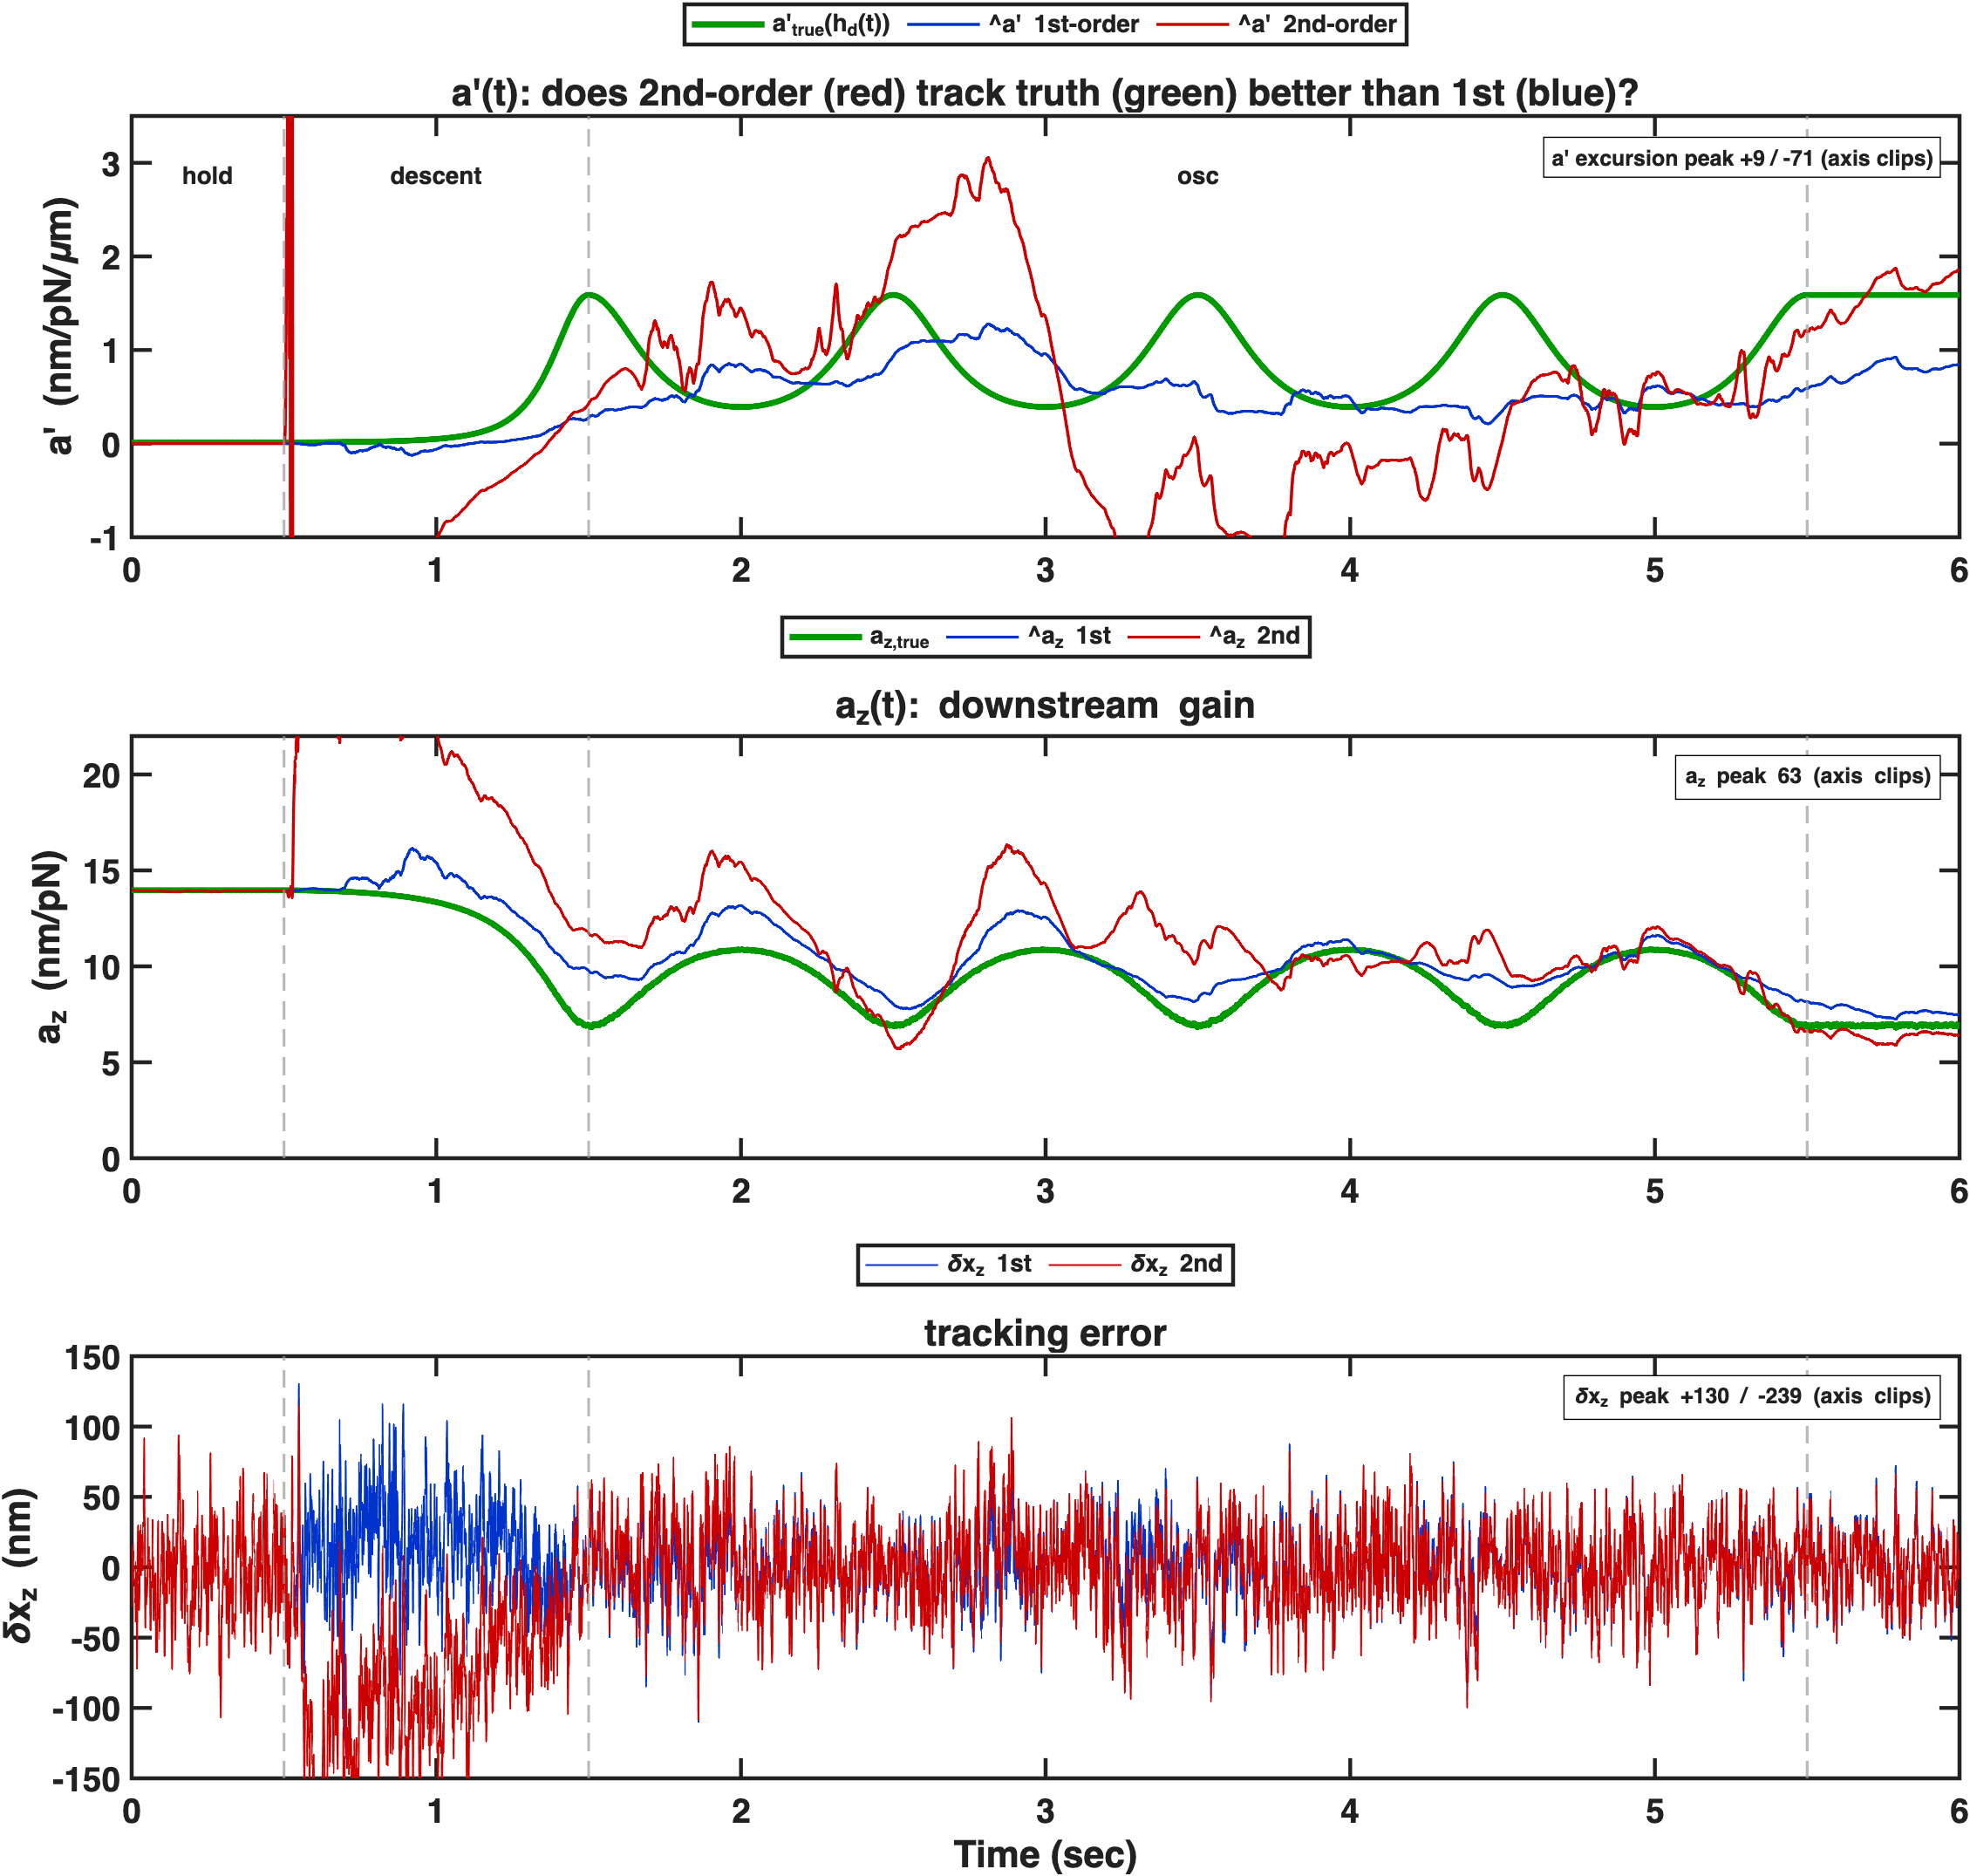
\includegraphics[width=0.96\textwidth]{figures/aprime_order_compare.png}
\end{center}
\begin{center}
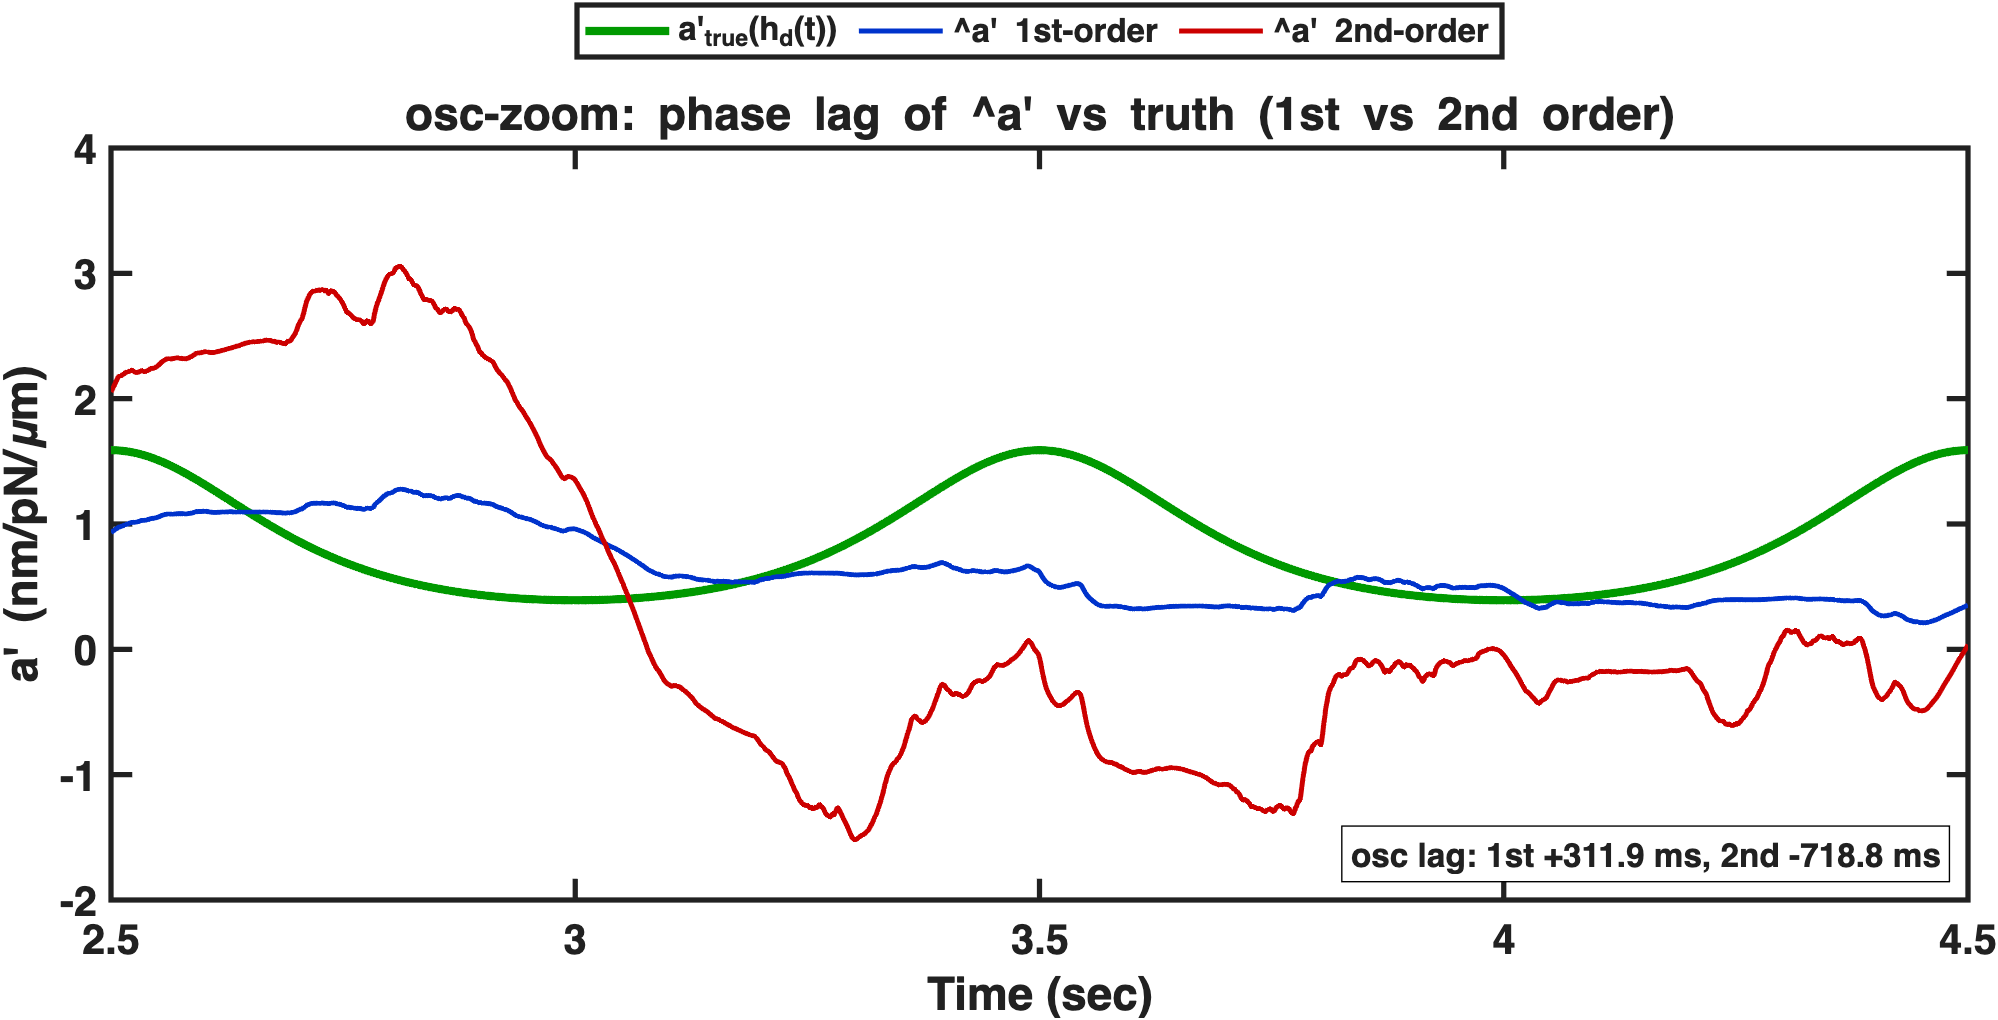
\includegraphics[width=0.96\textwidth]{figures/aprime_order_osc_zoom.png}
\end{center}
\textit{Canonical 1\,Hz, weak-obs as-state, seed 1, small $P_{55,0}$. osc $a'$ RMS: 2nd-order
$1.17$ vs 1st-order $0.55$; 1st-order tracks (lag $+312$\,ms), 2nd-order (IRW $\beta{=}1$)
wanders $-1.5$ to $+3$ (free integrator, $\va$ unobservable). $\hat a_z$ onset peak $63$,
$a'$ excursion $+9/{-}71$ (small $P_{55,0}$).}

\end{document}
